\subsection{Rys historyczny}

Dziedzina tej pracy, jaką jest przetwarzanie obrazów, ma początki swojej historii wcześniej niż urządzenia, które obecnie nazywamy komputerami.

\subsubsection{Wywoływanie zdjęć}
Przetwarzanie obrazów to nie jest technologia, która mogła zacząć istnieć po wynalezieniu komputerów. Używając aparatów korzystających z kliszy filmowej, po ekspozycji należy go poddać procesowi wywoływania (\autoref{fig:wywolywanie}). 
Polega on na wyciągnięciu pierwotnego efektu naświetlenia do obrazu, który oddaje scenę uchwyconą przez aparat \cite{doi:https://doi.org/10.1002/14356007.a20_001}. Proces w przypadku zdjęć aparatem na kliszę polega na zanurzaniu jej w odpowiednich związkach chemicznych na określone ilości czasu, by otrzymać zamierzony efekt. 

\begin{figure}[H]
    \centering
    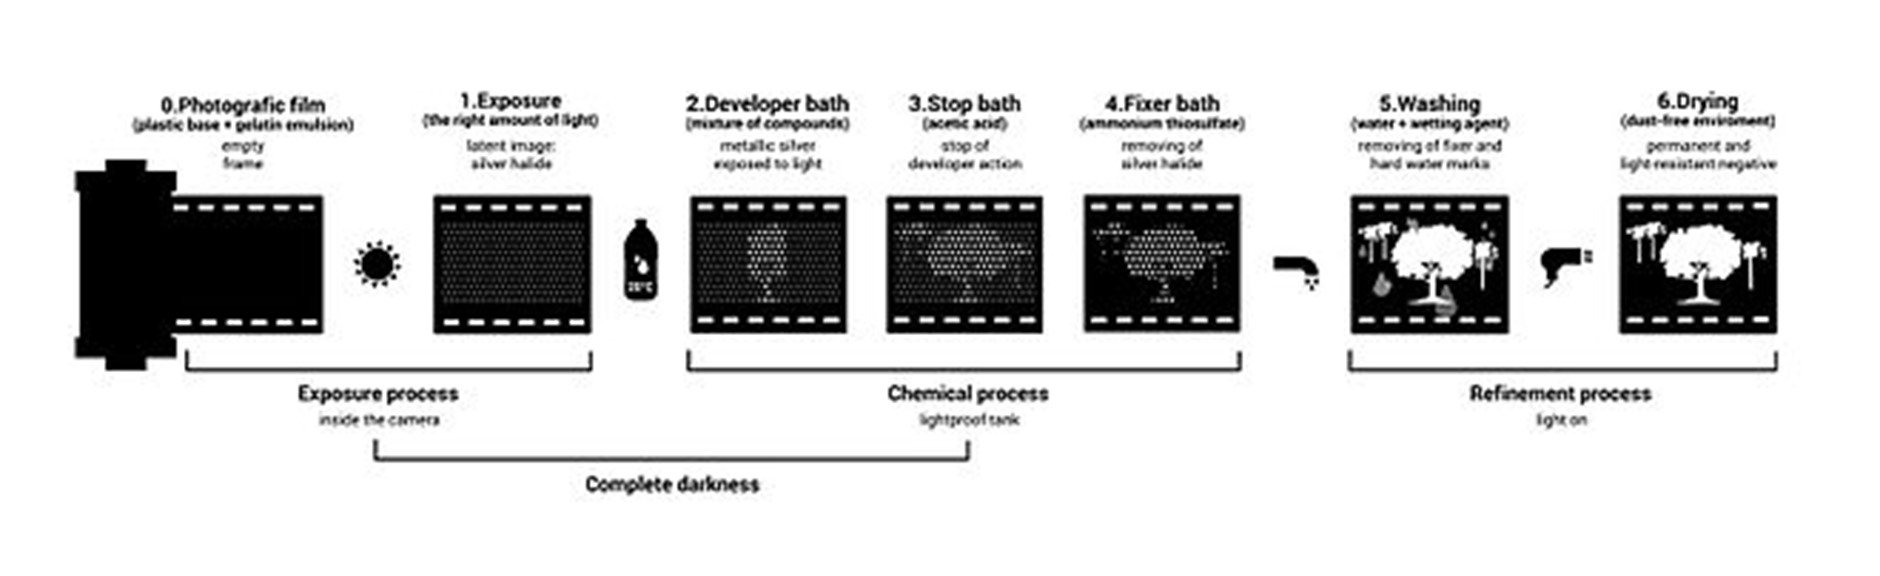
\includegraphics{./images/Picture1.jpg}
    \caption{Wywoływanie biało czarnej kliszy \cite{film}.}
    \label{fig:wywolywanie}
\end{figure}


Istnieją wariacje na temat takiego przetwarzania, różni się ono trochę w zależności od technologii kliszy. W niektórych przypadkach należy wywołać pozytyw zamiast negatywu \cite{almanac}. 
Następnie po wywoływaniu można poddać obróbce dalszymi chemikaliami jak np. siarczek sodu dla uzyskania efektu sepii \cite{sepia}. 

\subsubsection{Transmisja obrazów}
Technologia, którą znamy dobrze w obecnych czasach powstała w latach 20. XX wieku dzięki pracy John Logie Baird'a \cite{times1926}. 
Zaprezentował on pierwszą na świecie transmisję telewizyjną na żywo.
W 1928 roku \cite{bairdCompany} firma założona przez niego emitowała też pierwsze nagranie przez atlantyk. 
Wszystko to dzięki przetwarzaniu analogowego sygnału video w celu zmniejszenia ilości danych potrzebnych do wyświetlenia obrazu w telewizji \cite{analogVideo}.

\subsubsection{Cyfrowe przetwarzanie obrazów}
Początki nowoczesnego przetwarzania obrazów zostały stworzone w latach 60. XX w. w Bell Laboratories, Jet Propulsion Laboratory, Massachusetts Institute of Technology i University of Maryland \cite{computerProcessing}. 
Początkowymi obszarami zastosowania były obrazy satelitarne, przesyłanie obrazów przez linie telefoniczne, diagnostyka obrazowa, wideofony, rozpoznawanie znaków i ulepszanie fotografii. 

Inicjalnie dużo skupiano się na ulepszeniu jakości obrazu. Pierwszym znaczącym użyciem tych technologii było mapowanie powierzchni księżyca za pomocą zdjęć z sondy kosmicznej w 1964 roku, gdzie naukowcy z Jet Propulsion Laboratory na podstawie tysięcy zdjęć odtworzyli powierzchnię księżyca. 
Przy następnej okazji mieli dostęp do 100000 zdjęć, na podstawie których mogli stworzyć mapę topograficzną, mapę kolorową oraz panoramiczną mozaikę księżyca, które przyczyniły się do pierwszego lądowania człowieka na księżycu \cite{digitalImageProcessing}.

Technologia ta jednak była ograniczona przez bardzo małe możliwości oraz trudną dostępność komputerów tamtych czasów. 
Wraz z ich rozwojem i wzrostem popularności cyfrowe przetwarzanie obrazów przestało być trudno dostępną dziedziną naukową i stopniowo zostało wdrażane do naszego codziennego życia. 
Obecnie około 80\% populacji krajów rozwiniętych posiada smartfona \cite{smartphones}, który na swoim wyposażeniu ma kamerę cyfrową. 
Są one ograniczone poprzez fizyczny rozmiar matrycy oraz jakość soczewek, które mogą zmieścić się w telefonach komórkowych. 
Pomimo tego dzięki przetwarzaniu obrazów można uchwycić za ich pomocą imponujące zdjęcia \cite{pixel}. 
Nowoczesne telefony są w stanie zachować na zdjęciu nocnym detale, które może być ciężko zobaczyć ludzkim okiem \cite{nightMode} przez szybkie łączenie wielu obrazów o różnych długościach ekspozycji, redukcji szumów i korekcji kolorów.  

\subsection{Przegląd istniejących rozwiązań}

\subsubsection{Photoshop}
\begin{figure}[H]
    \centering
    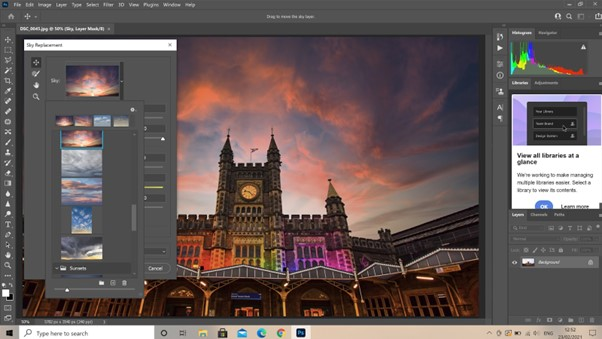
\includegraphics{./images/Picture2.jpg}
    \caption{Adobe Photoshop \cite{photoshop}.}
    \label{fig:photoshop}
\end{figure}

Wydany w 1990 roku do tworzenia i edytowania obrazów rastrowych jest jednym z najbardziej popularnych programów, a jego nazwa przedarła się do języka potocznego jako zamiennik dla fotomontażu. 
Użytkownikami tego oprogramowania są przeważnie artyści, fotografowie i twórcy internetowych memów. 
To narzędzie (\autoref{fig:photoshop}) jest przystosowane do łatwości obsługi przez mniej zaawansowanych użytkowników i wszystko posiada przyjazny graficzny interfejs użytkownika. 

Funkcje, które pozwalają na przetwarzanie obrazów często nie odnoszą się bezpośrednio do operacji zawartych w znanych bibliotekach do przetwarzania obrazów. 
Ich obsługa jest uproszczona i przystosowana do bardziej artystycznych zastosowań. 
Bez zastosowania szczególnej ostrożności - jak tworzenie nowych warstw po każdej operacji lub częste zapisywanie kopii zapasowej obrazu – przetwarzanie obrazów często jest destruktywne, nie możemy odnieść się do dowolnego momentu w ciągu naszych operacji w celu dopasowania jej parametrów. 
Przetwarzanie innego obrazu za pomocą tego samego procesu jest problematyczne, gdyż wymaga to ciągłego śledzenia warstw. Wiele operacji trzeba powtórzyć indywidualnie, ponieważ nie zapisujemy jej parametrów, tylko rezultat poprzedniego wykonania. Wiele bardziej zaawansowanych procesów nie jest możliwych do zrealizowania za pomocą standardowych opcji dostępnych w programie. Historia operacji jest też ograniczona i nie można wyświetlić pełnej historii na jednym ekranie - można jedynie zamieniać stan aktualny na wcześniejszy.

\subsubsection{ImageJ}
\begin{figure}[H]
    \centering
    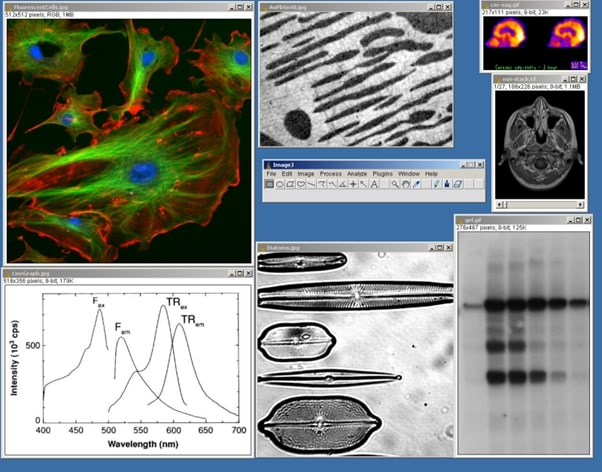
\includegraphics[width=0.8\linewidth]{./images/Picture3.jpg}
    \caption{ImageJ \cite{imagej}.}
    \label{fig:imagej}
\end{figure}

Wydany w 1997 roku program ImageJ (\autoref{fig:imagej}) został wykonany przez National Institutes of Health.Został on stworzony podstawowo z zamiarem analizy obrazów w zastosowaniach medycznych. 
Odtwarza dokładnie wiele operacji z bibliotek do przetwarzania obrazów i kod aplikacji jest otwartoźródłowy - każdy może go zobaczyć, pomóc w rozwoju lub stworzyć własną wersję. 
Napisany został w języku Java i ma bardzo niskie wymagania sprzętowe jak na obecne czasy.

Program jest jednak przestarzały, mogą pojawić się problemy z uruchomieniem na nowszych systemach. Interfejs użytkownika wygląda archaicznie oraz jego układ jest niepraktyczny biorąc pod uwagę przetwarzanie obrazów. 
Wszystkie operacje są schowane pod 1-2 poziomami menu. 
Operacje są destrukcyjne - zmieniają dane, które przetwarzamy więc to użytkownik musi pilnować aby mieć kopię swoich obrazów. 
Nie da się przygotować ciągów operacji wcześniej za pomocą interfejsu graficznego, trzeba użyć do tego ich języka programowania ImageJ Macro \cite{imagejbatch}. 
Od dawna nie jest rozwijany, został zastąpiony przez ImageJ2, który pozwala na przetwarzanie obrazów wielowymiarowych z dodatkowymi danymi np. z mikroskopów elektronowych, skanerów itp.

\subsubsection{Fiji}
\begin{figure}[H]
    \centering
    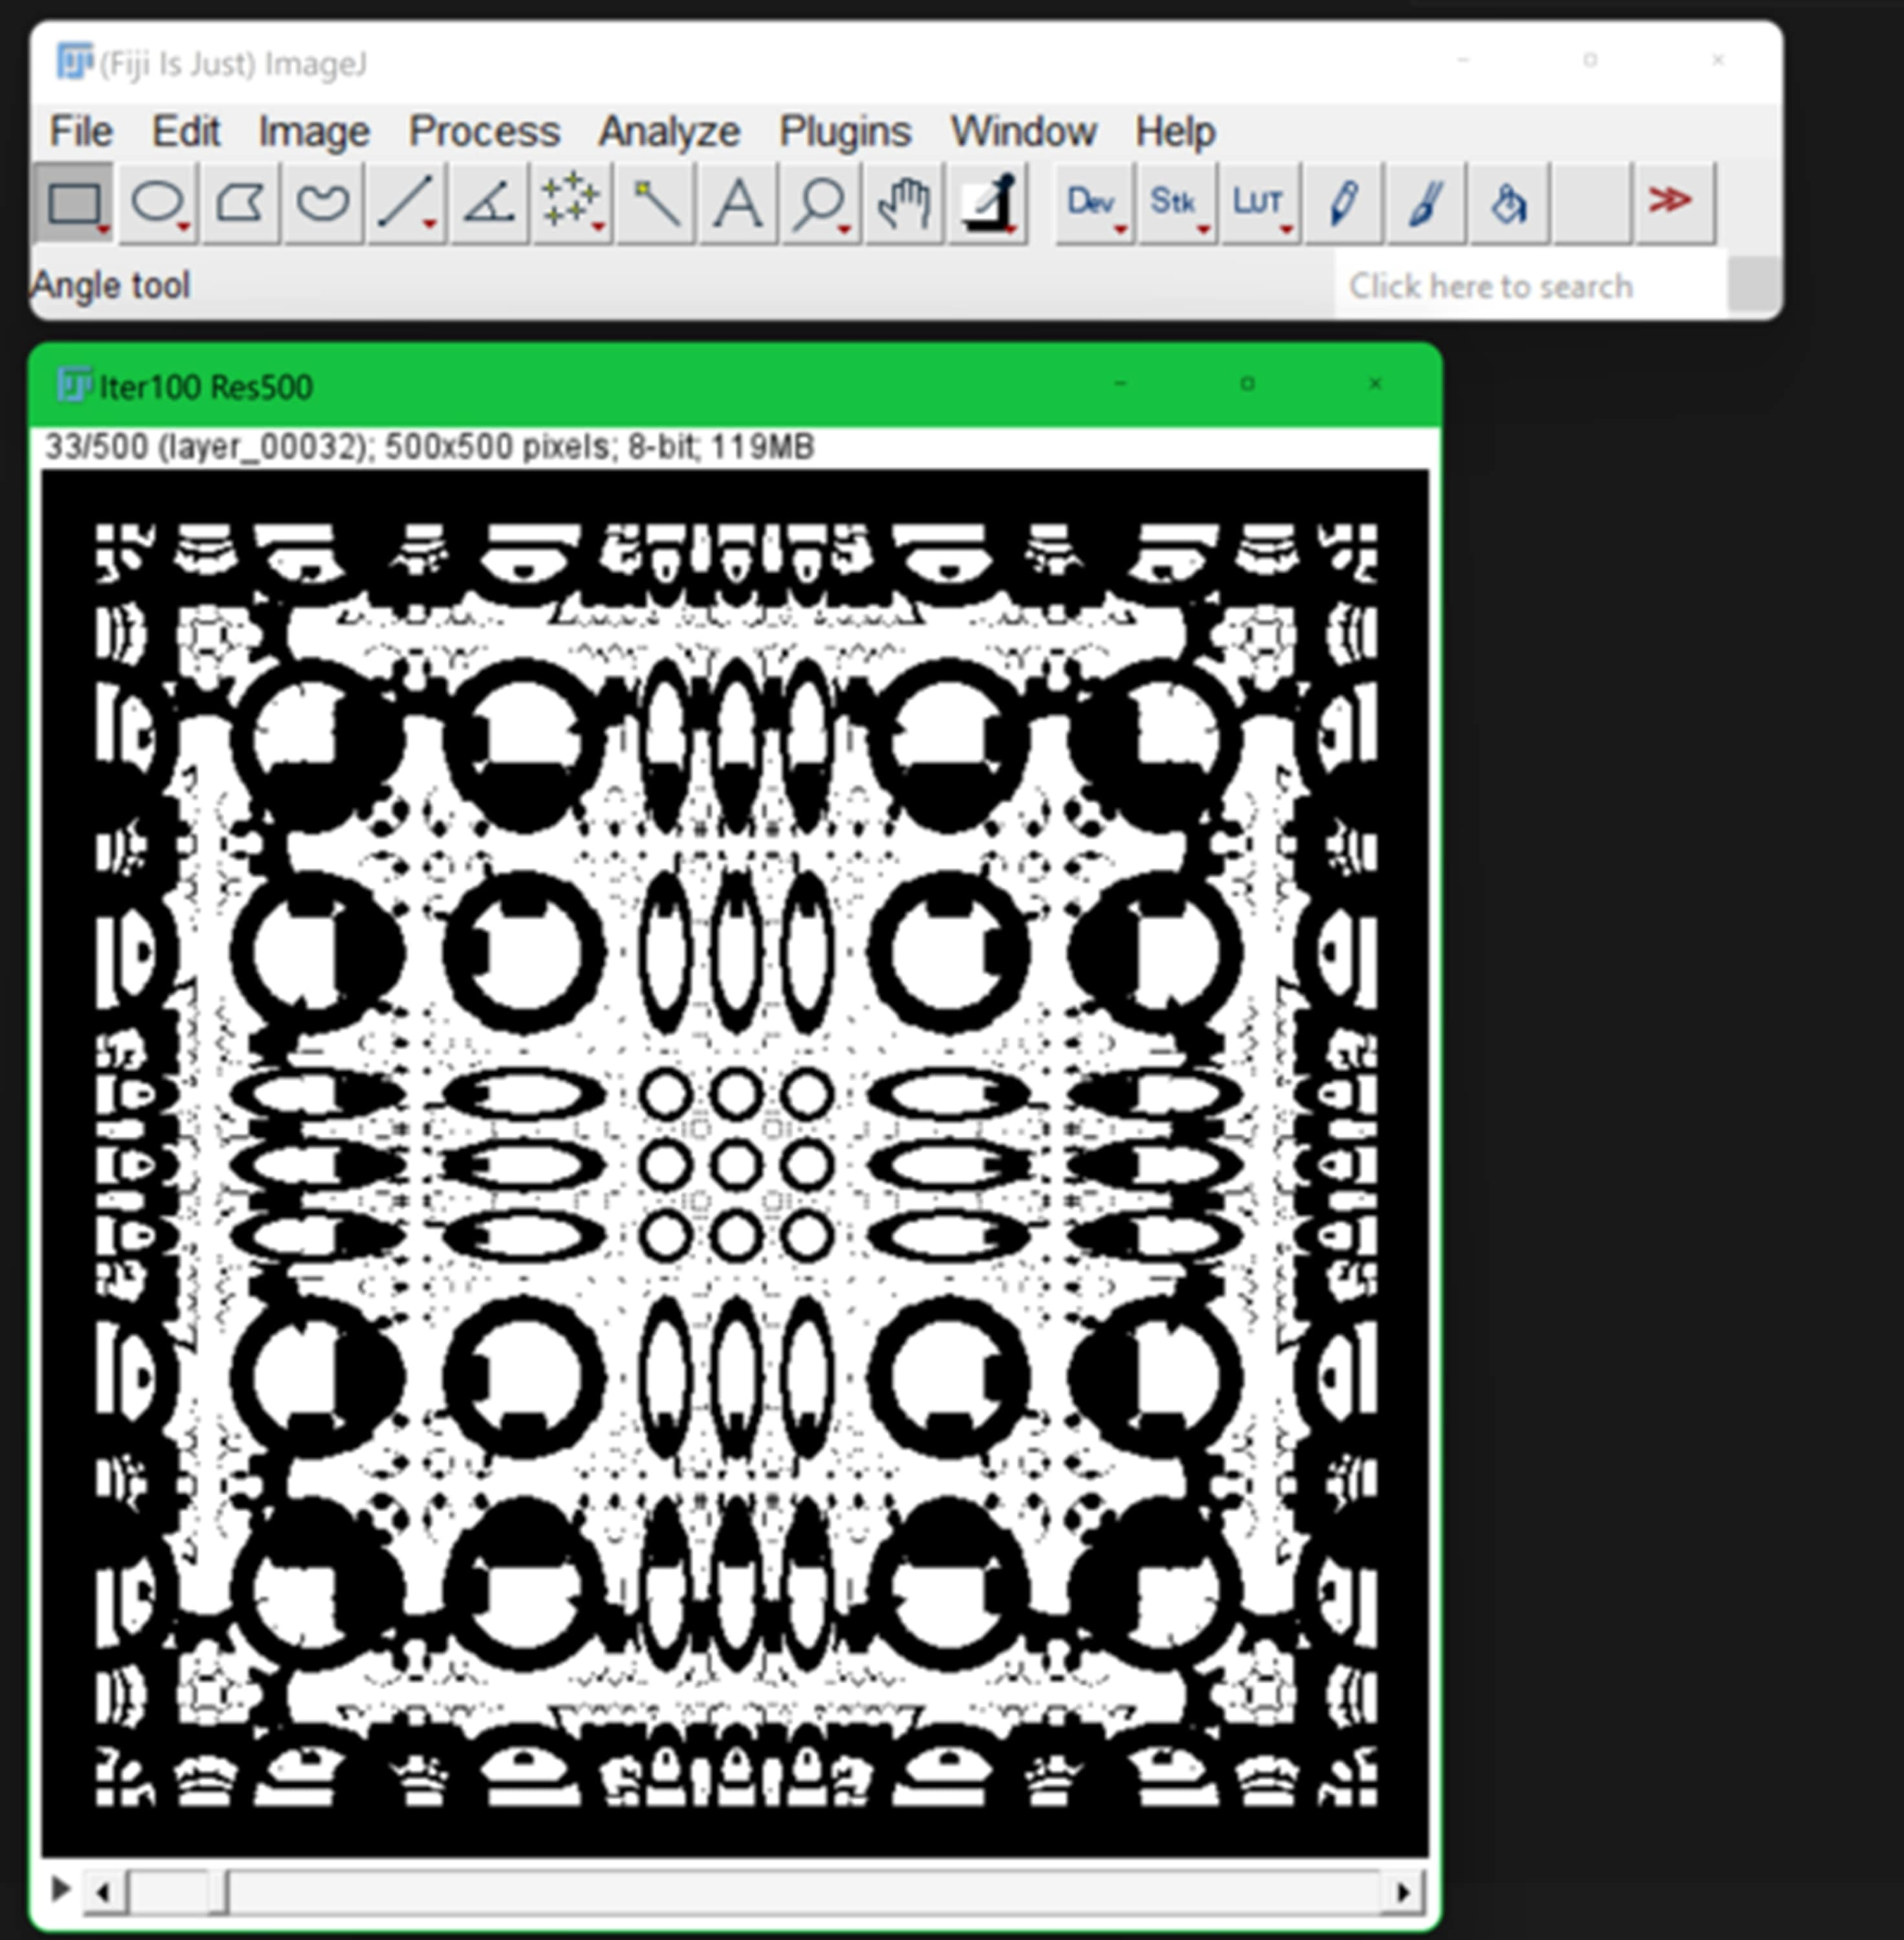
\includegraphics[width=0.8\linewidth]{./images/Picture4.jpg}
    \caption{Fiji - sukcesor ImageJ \cite{fiji}.}
    \label{fig:fiji}
\end{figure}

Projekt open source oparty o ImageJ2 (\autoref{fig:fiji}). Oprócz podstawowych operacji wbudowanych w ImageJ posiada też wiele pluginów znacząco rozszerzających możliwości programu. 
Są one skupione na wspomaganiu przetwarzania obrazów skupionych na dziedzinie neurobiologii, ale możliwości są na tyle szerokie, że wiele innych dziedzin nauki z niego korzysta.

Podstawowe działanie programu nie różni się od ImageJ więc, wszystkie jego problemy są też tutaj obecne. Jednakże poprawiona została jego kompatybilność z najnowszymi systemami operacyjnymi.

\subsubsection{GIMP}
\begin{figure}[H]
    \centering
    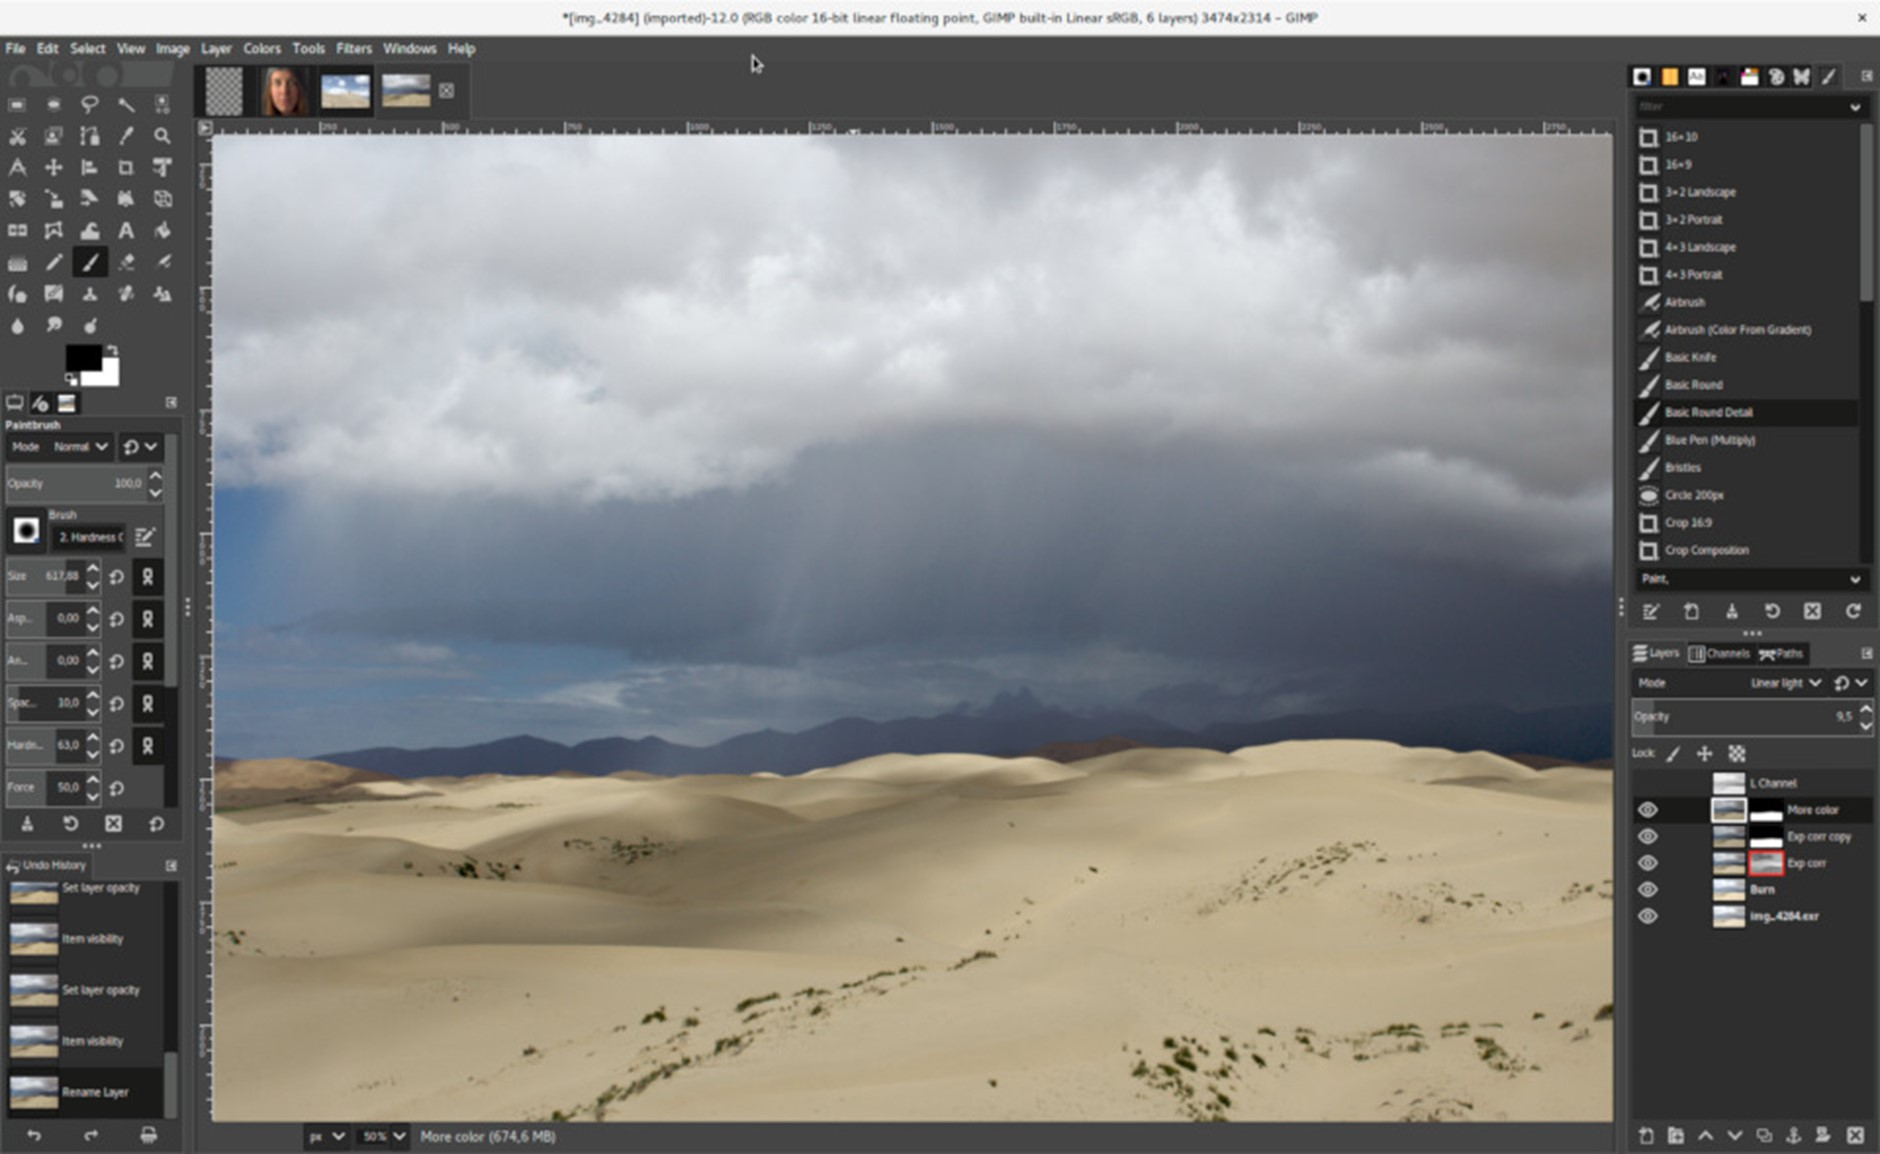
\includegraphics{./images/Picture5.jpg}
    \caption{GIMP wersja 2.10 \cite{gimp}.}
    \label{fig:gimp}
\end{figure}

Wydany w 1998 roku GNU Image Manipulation Program (\autoref{fig:gimp}) jest tworzony jako darmowa konkurencja dla Photoshopa, którego licencja jest miesięczną subskrypcją. Program też w pierwszej kolejności jest tworzony z myślą o artystach, ale posiada więcej zaawansowanych opcji jak np. konwolucje macierzowe, które można dowolnie edytować, dając duże możliwości filtrowania obrazów.

Pomimo odwzorowaniu większej liczby operacji ze standardowych bibliotek do przetwarzania obrazów i większej kontroli nad niektórymi z nich nadal występuje problem destruktywnego przetwarzania obrazów. Wynika to z pracy bezpośrednio na obrazie jak w Photoshopie i wymaga szczególnej uwagi przy zarządzaniu warstwami, aby nie tracić bezpowrotnie swoich pośrednich operacji w dłuższym ciągu.

\subsubsection{Adobe Substance Designer}
\begin{figure}[H]
    \centering
    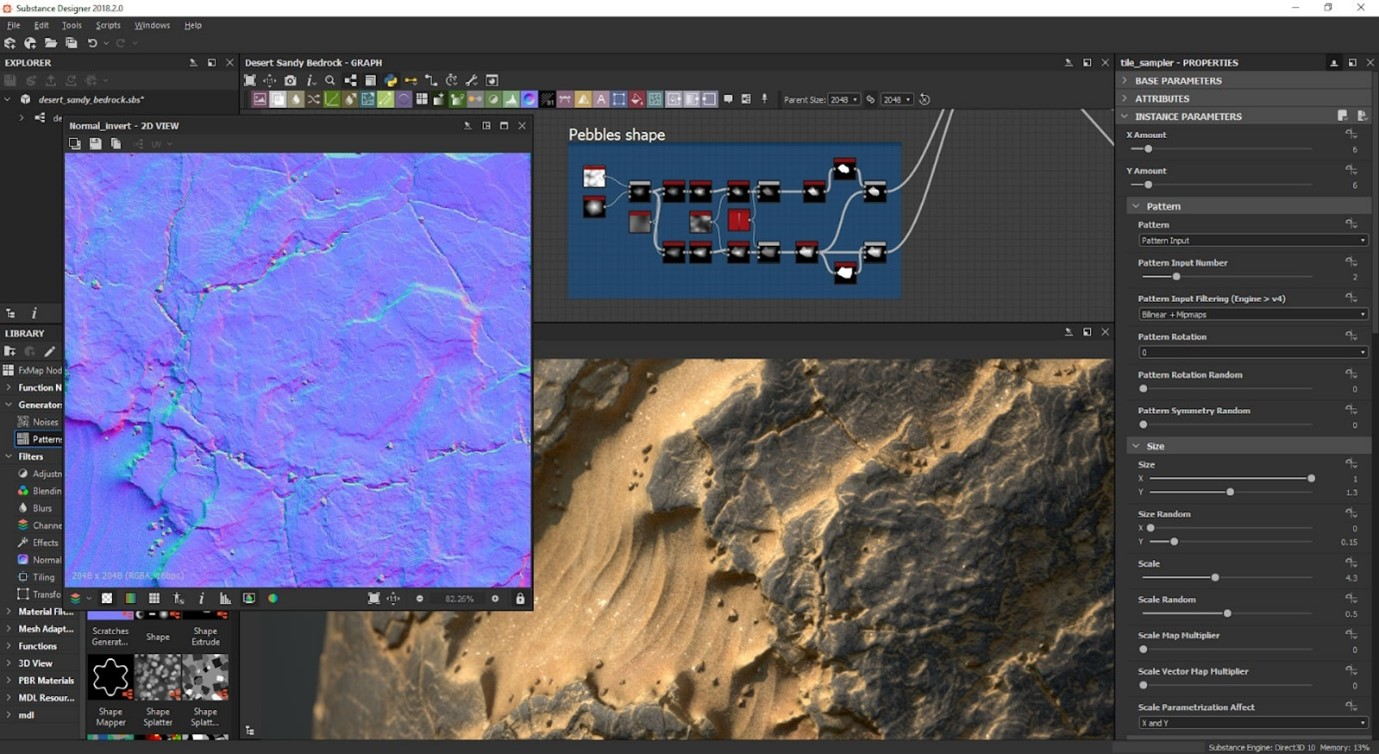
\includegraphics{./images/Picture6.jpg}
    \caption{Adobe Substance Designer \cite{designer}.}
    \label{fig:designer}
\end{figure}

Wydany w 2007 roku program (\autoref{fig:designer}) był główną inspiracją dla tego projektu. 
Jego dużą zaletą jest to, że tworzenie algorytmów bazuje na układaniu bloczków (nodów). 
Ułożony graf jest wykonywany na obrazie, który importujemy do programu lub generujemy go od początku w nim. 
Każdy dowolny node można kliknąć i zmienić wszystkie parametry jego operacji, niezależnie w którym miejscu ciągu on sie znajduje.
Jego wynik i wszystkie następne operacje, które są zależne od niego są obliczane ponownie na podstawie zmienionego wyniku. 
Zmiana przetwarzanego obrazu polega na przeciągnięciu połączenia z obecnego węzła z naszym plikiem wejściowym na nowy bloczek. Następnie propagowana jest zmiana na wszystkie kolejne operacje, których wynik jest aktualizowany automatycznie.

Opisywany program ten ma wiele ograniczeń związanych z tym, że nie jest stworzony do ogólnego przetwarzania obrazów. Został natomiast zaprojektowany do tworzenia materiałów/tekstur do grafiki komputerowej. 
Obrazy są ograniczone do boków o długości $2\textsuperscript{n}$, najlepiej kwadratowych. 
Parametry operacji są często uproszczone, ponieważ mimo większej złożoności aplikacji, jest ona nadal skierowana do artystów. 
Rodzaje operacji i wspierane formaty pikseli w pliku są przystosowane do wymagań grafiki komputerowej.
